\chapter{Desarrollo Analitico}

\section{Ejercicio 1}

El circuito a analizar consiste en una red de dos etapas RC en cascada. El análisis se realiza considerando el circuito
como una cadena de divisores resistivos en el dominio de Laplace (sin condiciones iniciales), tal como se muestra en la
Figura \ref{crkt.ej1:esquematico}.

\begin{figure}[!ht]
    \centering
    \begin{subfigure}[c]{0.45\textwidth}
        \centering
        \begin{circuitikz}[american]
    \draw (0,0) to[V, l=$V_i(s)$] (0,2)
    to[R, l=$R_1$] (2,2)
    to[C, l=$C_1$] (2,0) -- (0,0);
    \draw (2,2) to[R, l=$R_2$] (5,2)
    to[C, l=$C_2$, v=$V_o(s)$] (5,0) -- (2,0);
    \node at (2,2.3) {$V_1$};
\end{circuitikz}

    \end{subfigure}
    \hfill
    \begin{subfigure}[c]{0.45\textwidth}
        \begin{gather*}
            R_1 = 100 \si{\kilo\ohm} \quad C_1 = 91 \si{\pico\farad} \\
            R_2 = 182 \si{\kilo\ohm} \quad C_2 = 33 \si{\pico\farad}
        \end{gather*}
    \end{subfigure}
    \caption{red RC de dos etapas.}
    \label{crkt.ej1:esquematico}
\end{figure}


\subsection{Obtención de la Función de Transferencia}

Se plantea el análisis etapa por etapa, asumiendo independencia entre las mismas (despreciando el efecto de carga de la
segunda etapa sobre la primera):

\begin{equation}
    V_1 = \frac{V_i}{R_1 + \frac{1}{C_1 s}} \frac{1}{C_1 s}
\end{equation}

\begin{equation}
    V_o = \frac{V_1}{R_2 + \frac{1}{C_2 s}} \frac{1}{C_2 s}
\end{equation}
Sustituyendo $V_1$ en la expresión de $V_o$, obtenemos la función de transferencia $H(s)$:
{
\allowdisplaybreaks
\begin{align}
    V_o &= \frac{1}{R_2 + \frac{1}{C_2 s}} \frac{1}{C_2 s} \frac{V_i}{R_1 + \frac{1}{C_1 s}} \frac{1}{C_1 s} \nonumber \\[6pt] 
    H_{(s)} &= \frac{V_o}{V_i} = \frac{1}{R_2 + \frac{1}{C_2 s}} \frac{1}{C_2 s} \frac{1}{R_1 + \frac{1}{C_1 s}} \frac{1}{C_1 s} \nonumber \\[6pt]
    H_{(s)} &= \frac{1}{R_2 C_2 s + 1} \frac{1}{R_1 C_1 s + 1} \nonumber \\[6pt]
    H_{(s)} &= \frac{1}{R_1 R_2 C_1 C_2} \frac{1}{s + \frac{1}{R_2 C_2}} \frac{1}{s + \frac{1}{R_1 C_1}} \nonumber \\[6pt]
    H_{(s)} &=  \frac{\frac{1}{R_1 R_2 C_1 C_2}}{\left(s + \frac{1}{R_2 C_2}\right) \left(s + \frac{1}{R_1 C_1}\right)}
    \label{eq.ej1:fdt_simbolica}
\end{align}
}
Substituyendo numericamente obtenemos:
\begin{equation}
    H_{(s)} =  \frac{18,\!2967 \times 10^9}{\left(s + 166500,\!1665\right) \left(s + 109890,\!1099\right)}
    \label{eq.ej1:fdt_numerica}
\end{equation}

\subsection{Valor de continua, ceros y polos}

La componente de continua del sistema se puede obtener normalizando la funcion de transferencia \ref{eq.ej1:fdt_numerica} de
forma que queden los polos y ceros de la forma $ks \pm 1$. Haciendo $20\log_{10}\left(K_{te}\right)$ podemos obtener la
componente de continua del sistema:

\begin{align*}
    K_{te} &= 20 log_{10}\left(18,\!2967 \times 10^9 \cdot \frac{1}{166500,\!1665} \cdot \frac{1}{109890,\!1099}\right) \\[6pt]
    K_{te} &= -10,\!25 \times 10^{-6} \si{\decibel} \approx 0 \si{\decibel}
\end{align*}

El sistema carece de ceros. Los polos del sistema se encuentran en:
\begin{align*}
    \omega &= 166500,\!1665 \approx 1,\!6 \times 10^5 \si{\radian\per\second} \\[6pt]
    \omega &= 109890,\!1099 \approx 10^5 \si{\radian\per\second}
\end{align*}


\subsection{Analisis fasorial}

Para obtener la respuesta en frecuencia de forma polar, pasamos a la forma fasorial haciendo $s \to j\omega$. Partiendo
de \ref{eq.ej1:fdt_simbolica}, multiplicando los polos y la constante del numerador, obtenemos:

\begin{equation}
    H(j\omega) = \frac{1}{(1 - \omega^2 R_1 R_2 C_1 C_2) + j\omega(R_1 C_1 + R_2 C_2)}
\end{equation}
Para separar las partes real e imaginaria, multiplicamos y dividimos por el conjugado del denominador:
\begin{equation*}
    H(j\omega) = \frac{(1 - \omega^2 R_1 R_2 C_1 C_2) - j\omega(R_1 C_1 + R_2 C_2)}{(1 - \omega^2 R_1 R_2 C_1 C_2)^2 + \omega^2(R_1 C_1 + R_2 C_2)^2}
\end{equation*}
De donde se obtienen las expresiones para el análisis del diagrama polar:
\begin{align}
    \Re\left\{H_{(j\omega)}\right\} &= \frac{1 - \omega^2 R_1 R_2 C_1 C_2}{(1 - \omega^2 R_1 R_2 C_1 C_2)^2 + \omega^2(R_1 C_1 + R_2 C_2)^2} \nonumber \\[6pt]
    \Re\left\{H_{(j\omega)}\right\} &= \frac{1 - \omega^2 54,\!65 \times 10^{-12}}{(1 - \omega^2 54,\!65 \times 10^{-12})^2 + \omega^2 (9,\!1 \times 10^{-6} + 6 \times 10^{-6})^2}
    \label{eq.ej1:re_h}
\end{align}

\begin{align}
    \Im\left\{H_{(j\omega)}\right\} &= \frac{-\omega(R_1 C_1 + R_2 C_2)}{(1 - \omega^2 R_1 R_2 C_1 C_2)^2 + \omega^2(R_1 C_1 + R_2 C_2)^2} \nonumber \\[6pt]
    \Im\left\{H_{(j\omega)}\right\} &= \frac{- \omega (9,\!1 \times 10^{-6} + 6 \times 10^{-6})}{(1 - \omega^2 54,\!65 \times 10^{-12})^2 + \omega^2 (9,\!1 \times 10^{-6} + 6 \times 10^{-6})^2}
    \label{eq.ej1:im_h}
\end{align}

\subsection{Diagrama Polar}

Para trazar el diagrama polar, se evalúan las ecuaciones \ref{eq.ej1:re_h} e \ref{eq.ej1:im_h} para diferentes valores de
frecuencia angular $\omega$. Los resultados se resumen en la Tabla \ref{tab.ej1:puntos_polar} y la figura
\ref{fig.ej1:polar_hand}.

\begin{figure}[!ht]
    \centering
    \begin{subfigure}[c]{0.45\textwidth}
        \centering
        \resizebox{\textwidth}{!}{
            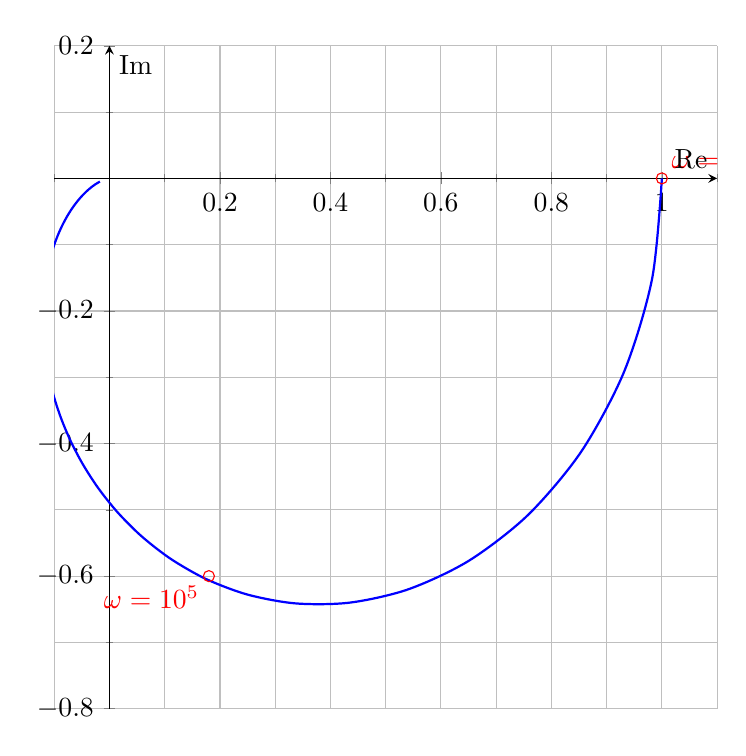
\begin{tikzpicture}
    \begin{axis}[
        xlabel={Re},
        ylabel={Im},
        grid=both,
        width=10cm,
        height=10cm,
        xmin=-0.1, xmax=1.1,
        ymin=-0.8, ymax=0.2,
        axis lines=middle,
        minor tick num=1,
        samples=100,
    ]
        \addplot[blue, thick, smooth, domain=0:10] ({
            (1 - x^2 * 0.5465) / ((1 - x^2 * 0.5465)^2 + x^2 * (1.5106)^2)
        }, {
            (-x * 1.5106) / ((1 - x^2 * 0.5465)^2 + x^2 * (1.5106)^2)
        });
        
        \addplot[only marks, red, mark=o] coordinates {(1,0)} node[above right] {$\omega=0$};
        \addplot[only marks, red, mark=o] coordinates {(0.18,-0.6)} node[below left] {$\omega=10^5$};
    \end{axis}
\end{tikzpicture}

        }
        \caption{diagrama polar.}
        \label{fig.ej1:polar_hand}
    \end{subfigure}
    \hfill
    \begin{subfigure}[c]{0.45\textwidth}
        \centering
        \begin{tabular}{|c|c|c|}
            \hline
            $\omega$ [\SI{}{\radian\per\second}] & $\text{Re}\{H(j\omega)\}$ & $\text{Im}\{H(j\omega)\}$ \\ \hline
            0 & 1 & 0 \\ \hline
            1 & 0,99 & $\approx 0$ \\ \hline
            $10^4$ & 0,98 & -0,14 \\ \hline
            $2 \cdot 10^4$ & 0,93 & -0,28 \\ \hline
            $3 \cdot 10^4$ & 0,85 & -0,4 \\ \hline
            $5 \cdot 10^4$ & 0,65 & -0,57 \\ \hline
            $7 \cdot 10^4$ & 0,44 & -0,63 \\ \hline
            $9 \cdot 10^4$ & 0,25 & -0,62 \\ \hline
            $10^5$ & 0,18 & -0,6 \\ \hline
        \end{tabular}
        \caption{puntos calculados para el diagrama.}
        \label{tab.ej1:puntos_polar}
    \end{subfigure}
    \caption{analisis polar.}
\end{figure}

\subsection{Diagrama de Bode}

En la Figura \ref{fig.ej1:bode_octave} se presentan los diagramas de magnitud y fase generados mediante la herramienta
\texttt{Octave}, utilizando la biblioteca \texttt{bodas} \cite{bodas}. Estos gráficos corroboran los resultados
del desarrollo analítico realizado manualmente (cuyo registro se encuentra en el Anexo \ref{sec.ej1:anexo_papel}).

\begin{figure}[!ht]
    \centering
    \begin{subfigure}[t]{\textwidth}
        \centering
        % Title: Magnitude: Asymptotic with Parts
% Creator: GL2PS 1.4.2, (C) 1999-2020 C. Geuzaine
% For: Octave
% CreationDate: Thu Jun 18 20:42:31 2026
\setlength{\unitlength}{1pt}
\begin{picture}(0,0)
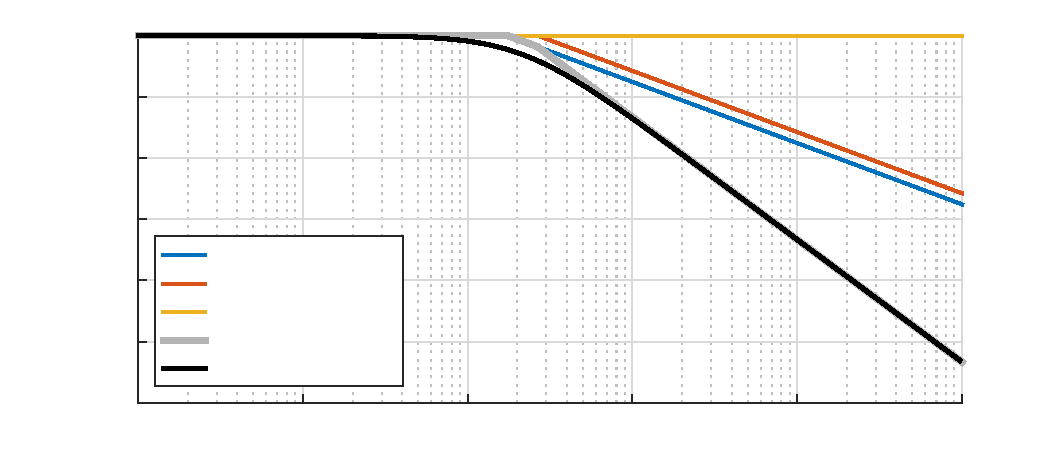
\includegraphics[scale=1]{figures/plot_ej1_bodas_gain-inc}
\end{picture}%
\begin{picture}(510,226)(0,0)
\fontsize{10}{0}\selectfont\put(66.3307,25.2292){\makebox(0,0)[t]{\textcolor[rgb]{0.15,0.15,0.15}{{$10^{2}$}}}}
\fontsize{10}{0}\selectfont\put(145.417,25.2292){\makebox(0,0)[t]{\textcolor[rgb]{0.15,0.15,0.15}{{$10^{3}$}}}}
\fontsize{10}{0}\selectfont\put(224.504,25.2292){\makebox(0,0)[t]{\textcolor[rgb]{0.15,0.15,0.15}{{$10^{4}$}}}}
\fontsize{10}{0}\selectfont\put(303.591,25.2292){\makebox(0,0)[t]{\textcolor[rgb]{0.15,0.15,0.15}{{$10^{5}$}}}}
\fontsize{10}{0}\selectfont\put(382.677,25.2292){\makebox(0,0)[t]{\textcolor[rgb]{0.15,0.15,0.15}{{$10^{6}$}}}}
\fontsize{10}{0}\selectfont\put(461.764,25.2292){\makebox(0,0)[t]{\textcolor[rgb]{0.15,0.15,0.15}{{$10^{7}$}}}}
\fontsize{10}{0}\selectfont\put(61.3252,32.74){\makebox(0,0)[r]{\textcolor[rgb]{0.15,0.15,0.15}{{-120}}}}
\fontsize{10}{0}\selectfont\put(61.3252,62.1153){\makebox(0,0)[r]{\textcolor[rgb]{0.15,0.15,0.15}{{-100}}}}
\fontsize{10}{0}\selectfont\put(61.3252,91.4907){\makebox(0,0)[r]{\textcolor[rgb]{0.15,0.15,0.15}{{-80}}}}
\fontsize{10}{0}\selectfont\put(61.3252,120.866){\makebox(0,0)[r]{\textcolor[rgb]{0.15,0.15,0.15}{{-60}}}}
\fontsize{10}{0}\selectfont\put(61.3252,150.241){\makebox(0,0)[r]{\textcolor[rgb]{0.15,0.15,0.15}{{-40}}}}
\fontsize{10}{0}\selectfont\put(61.3252,179.617){\makebox(0,0)[r]{\textcolor[rgb]{0.15,0.15,0.15}{{-20}}}}
\fontsize{10}{0}\selectfont\put(61.3252,208.992){\makebox(0,0)[r]{\textcolor[rgb]{0.15,0.15,0.15}{{0}}}}
\fontsize{11}{0}\selectfont\put(264.047,11.2292){\makebox(0,0)[t]{\textcolor[rgb]{0.15,0.15,0.15}{{Frequency (Hz)}}}}
\fontsize{11}{0}\selectfont\put(38.3252,120.866){\rotatebox{90}{\makebox(0,0)[b]{\textcolor[rgb]{0.15,0.15,0.15}{{Magnitude (dB)}}}}}
\fontsize{9}{0}\selectfont\put(102.378,103.777){\makebox(0,0)[l]{\textcolor[rgb]{0,0,0}{{1/(1 + s/109890.1099)}}}}
\fontsize{9}{0}\selectfont\put(102.378,89.7715){\makebox(0,0)[l]{\textcolor[rgb]{0,0,0}{{1/(1 + s/166500.1665)}}}}
\fontsize{9}{0}\selectfont\put(102.378,76.2663){\makebox(0,0)[l]{\textcolor[rgb]{0,0,0}{{K = -1.0252e-05 dB}}}}
\fontsize{9}{0}\selectfont\put(102.378,62.761){\makebox(0,0)[l]{\textcolor[rgb]{0,0,0}{{Asymptotic Sum}}}}
\fontsize{9}{0}\selectfont\put(102.378,49.2558){\makebox(0,0)[l]{\textcolor[rgb]{0,0,0}{{Exact Bode}}}}
\end{picture}

    \end{subfigure}
    \begin{subfigure}[b]{\textwidth}
        \centering
        \vspace{-1cm}
        % Title: Phase: Asymptotic with Parts
% Creator: GL2PS 1.4.2, (C) 1999-2020 C. Geuzaine
% For: Octave
% CreationDate: Sun May 31 17:23:09 2026
\setlength{\unitlength}{1pt}
\begin{picture}(0,0)
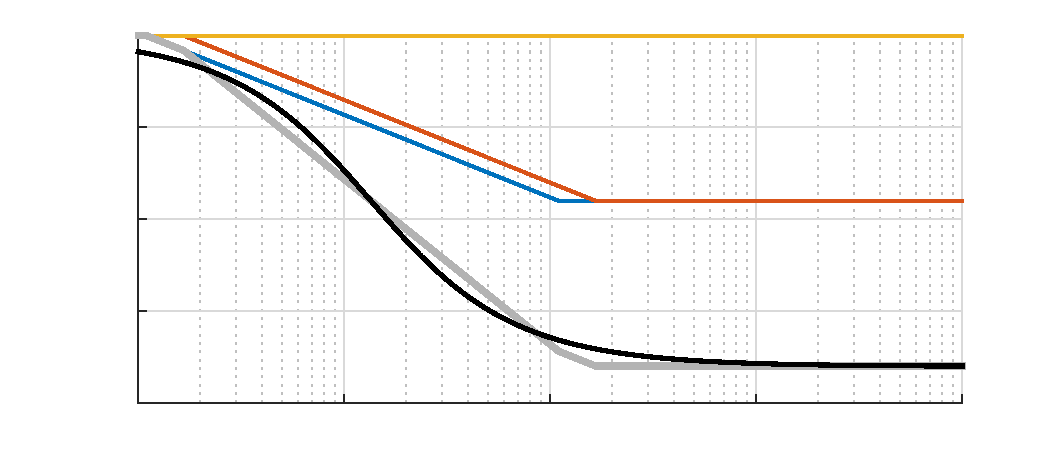
\includegraphics[scale=1]{figures/plot_ej1_bodas_phase-inc}
\end{picture}%
\begin{picture}(510,226)(0,0)
\fontsize{10}{0}\selectfont\put(66.3307,25.2292){\makebox(0,0)[t]{\textcolor[rgb]{0.15,0.15,0.15}{{$10^{4}$}}}}
\fontsize{10}{0}\selectfont\put(165.189,25.2292){\makebox(0,0)[t]{\textcolor[rgb]{0.15,0.15,0.15}{{$10^{5}$}}}}
\fontsize{10}{0}\selectfont\put(264.047,25.2292){\makebox(0,0)[t]{\textcolor[rgb]{0.15,0.15,0.15}{{$10^{6}$}}}}
\fontsize{10}{0}\selectfont\put(362.906,25.2292){\makebox(0,0)[t]{\textcolor[rgb]{0.15,0.15,0.15}{{$10^{7}$}}}}
\fontsize{10}{0}\selectfont\put(461.764,25.2292){\makebox(0,0)[t]{\textcolor[rgb]{0.15,0.15,0.15}{{$10^{8}$}}}}
\fontsize{10}{0}\selectfont\put(61.3252,32.74){\makebox(0,0)[r]{\textcolor[rgb]{0.15,0.15,0.15}{{-200}}}}
\fontsize{10}{0}\selectfont\put(61.3252,76.803){\makebox(0,0)[r]{\textcolor[rgb]{0.15,0.15,0.15}{{-150}}}}
\fontsize{10}{0}\selectfont\put(61.3252,120.866){\makebox(0,0)[r]{\textcolor[rgb]{0.15,0.15,0.15}{{-100}}}}
\fontsize{10}{0}\selectfont\put(61.3252,164.929){\makebox(0,0)[r]{\textcolor[rgb]{0.15,0.15,0.15}{{-50}}}}
\fontsize{10}{0}\selectfont\put(61.3252,208.992){\makebox(0,0)[r]{\textcolor[rgb]{0.15,0.15,0.15}{{0}}}}
\fontsize{11}{0}\selectfont\put(264.047,11.2292){\makebox(0,0)[t]{\textcolor[rgb]{0.15,0.15,0.15}{{Frequency (rad/s)}}}}
\fontsize{11}{0}\selectfont\put(38.3252,120.866){\rotatebox{90}{\makebox(0,0)[b]{\textcolor[rgb]{0.15,0.15,0.15}{{Phase (degrees)}}}}}
\end{picture}

    \end{subfigure}
    \caption{Diagramas de Bode (Magnitud y Fase) generados con Octave.}
    \label{fig.ej1:bode_octave}
\end{figure}

\subsection{Simulación y Comparación}

Para validar los resultados teóricos y de cálculo, se realizó una simulación del circuito en \texttt{KiCad} utilizando
el análisis de pequeña señal (AC). En la Figura \ref{fig.ej1:simulacion_kicad} se observa la respuesta en frecuencia
obtenida, la cual presenta una total coincidencia con los gráficos anteriormente analizados.

\begin{figure}[!ht]
    \centering
    \begin{tikzpicture}
    \pgfplotsset{
        nice plot/.style={
            /pgf/number format/read comma as period,
            grid=both,
            major grid style={solid, gray!50},
            minor grid style={dotted, gray!50},
            axis line style={black},
            axis x line* = bottom,
            axis y line* = left,
            extra description/.code={
                \draw[gray!50] (rel axis cs:0,1) -- (rel axis cs:1,1) -- (rel axis cs:1,0);
            },
            width=16cm,
            height=8cm,
            xmin=1e2, xmax=1e7,
            minor x tick num=9,
            minor y tick num=0,
        }
    }

    \begin{semilogxaxis}[
        nice plot,
        ylabel={A [dB]},
        ymin=-120, ymax=0,
    ]
        \addplot[thick, blue] table [x expr=\thisrow{frequency}, y={V(/Vo) (ganancia)}, col sep=semicolon] {sources/plots/tdc2_tp1_ej1};
    \end{semilogxaxis}

    \begin{semilogxaxis}[
        nice plot,
        xlabel={$\omega$ [Hz]},
        ylabel={$\phi$ [º]},
        ymin=-200, ymax=0,
        at={(0,-8.5cm)},
    ]
        \addplot[thick, red] table [x expr=\thisrow{frequency}, y={V(/Vo) (fase)}, col sep=semicolon] {sources/plots/tdc2_tp1_ej1};
    \end{semilogxaxis}
\end{tikzpicture}

    \caption{Respuesta en frecuencia simulada.}
    \label{fig.ej1:simulacion_kicad}
\end{figure}

\clearpage

\section{Ejercicio 2}

El circuito a analizar consiste en una red RLC que se comporta como un filtro rechaza-banda. El análisis se
realiza en el dominio de Laplace (sin condiciones iniciales) considerando el circuito como un divisor de tensión,
tal como se muestra en la Figura \ref{crkt.ej2:esquematico}.

\begin{figure}[!ht]
    \centering
    \begin{subfigure}[c]{0.45\textwidth}
        \centering
        \begin{circuitikz}[american]
    \draw (0,4) to[V, l=$V_i(s)$] (0,0);
    \draw (0,4) to[R, l=$R$] (4,4)
    to[L, l=$L$] (4,2)
    to[C, l=$C$] (4,0) -- (0,0);
    \draw (4,4) to[short, -*] (4.8,4) node[above] {$V_o(s)$};
    \node[ground] at (4,0) {};
\end{circuitikz}

    \end{subfigure}
    \hfill
    \begin{subfigure}[c]{0.45\textwidth}
        \begin{gather*}
            R = 100 \si{\kilo\ohm} \\
            C = 3,\!18 \si{\micro\farad} \\
            L = 31,\!83 \si{\milli\henry}
        \end{gather*}
    \end{subfigure}
    \caption{Red RLC rechaza-banda.}
    \label{crkt.ej2:esquematico}
\end{figure}


\subsection{Obtención de la Función de Transferencia}

La impedancia de la rama en derivación (shunt), formada por la conexión en serie del inductor $L$ y el capacitor $C$,
se plantea como:
\begin{equation}
    Z_{LC}(s) = L s + \frac{1}{C s} = \frac{L C s^2 + 1}{C s}
\end{equation}

Aplicando el divisor de tensión, la tensión de salida $V_o(s)$ en función de la tensión de entrada $V_i(s)$ resulta:
\begin{equation}
    V_o(s) = V_i(s) \frac{Z_{LC}(s)}{R + Z_{LC}(s)}
\end{equation}

Sustituyendo $Z_{LC}(s)$ obtenemos la función de transferencia simbólica $H(s)$:
{
\allowdisplaybreaks
\begin{align}
    H(s) &= \frac{V_o(s)}{V_i(s)} = \frac{\frac{L C s^2 + 1}{C s}}{R + \frac{L C s^2 + 1}{C s}} \nonumber \\[6pt]
    H(s) &= \frac{L C s^2 + 1}{L C s^2 + R C s + 1} \nonumber \\[6pt]
    H(s) &= \frac{s^2 + \frac{1}{LC}}{s^2 + \frac{R}{L} s + \frac{1}{LC}}
    \label{eq.ej2:fdt_simbolica}
\end{align}
}

Sustituyendo numéricamente con los valores asignados:
\begin{align*}
    L C &= 31,\!83 \times 10^{-3} \si{\henry} \times 3,\!18 \times 10^{-6} \si{\farad} \\
    &\approx 1,\!012194 \times 10^{-7} \si{\second\squared} \\[6pt]
    R C &= 100 \si{\kilo\ohm} \times 3,\!18 \si{\micro\farad} = 0,\!318 \si{\second} \\[6pt]
    \frac{R}{L} &= \frac{100 \si{\kilo\ohm}}{31,\!83 \si{\milli\henry}} \\
    &\approx 3,\!14169 \times 10^6 \si{\radian\per\second} \\[6pt]
    \frac{1}{LC} &= \omega_0^2 \approx 9,\!8795 \times 10^6 \si{\radian\squared\per\second\squared}
\end{align*}

Reemplazando estos coeficientes en la ecuación \ref{eq.ej2:fdt_simbolica}, se obtiene la función de transferencia
numérica:
\begin{equation}
    H(s) = \frac{s^2 + 9,\!8795 \times 10^6}{s^2 + 3,\!1417 \times 10^6 s + 9,\!8795 \times 10^6}
    \label{eq.ej2:fdt_numerica}
\end{equation}


\subsection{Valor de continua, ceros y polos}

El valor de ganancia en continua (DC) se calcula evaluando la función de transferencia en $s = 0$:
\begin{equation*}
    H(0) = \frac{9,\!8795 \times 10^6}{9,\!8795 \times 10^6} = 1 \implies 20\log_{10}(1) = 0 \si{\decibel}
\end{equation*}

De igual manera, el límite de alta frecuencia ($s \to \infty$) tiende a la unidad:
\begin{equation*}
    \lim_{s \to \infty} H(s) = 1
\end{equation*}
Los ceros de la función de transferencia se calculan igualando el numerador a cero:
\begin{equation}
    N(s) = s^2 + \omega_0^2 = 0
\end{equation}
De aquí se obtiene de forma directa un par de ceros conjugados ubicados en el eje imaginario:
\begin{equation}
    s_{z1,z2} = \pm j \omega_0
\end{equation}
Reemplazando con los valores de $L$ y $C$:
\begin{align*}
    s_{z1,z2} &= \pm j \frac{1}{\sqrt{31,\!83 \si{\milli\henry} \times 3,\!18 \si{\micro\farad}}} \\
    &= \pm j \frac{1}{\sqrt{1,\!012194 \times 10^{-7} \si{\second\squared}}} \\
    &\approx \pm j 3143,\!17 \si{\radian\per\second}
\end{align*}
Esto define una frecuencia de resonancia de:
\begin{equation*}
    f_0 = \frac{\omega_0}{2\pi} \approx 500,\!25 \si{\hertz}
\end{equation*}
En esta frecuencia, la ganancia teórica de tensión se anula por completo ($-\infty \si{\decibel}$).

Los polos corresponden a las raíces del polinomio del denominador:
\begin{equation}
    D(s) = s^2 + \frac{R}{L}s + \omega_0^2 = 0
\end{equation}
Sustituyendo los valores numéricos correspondientes a los componentes:
\begin{equation}
    s^2 + 3,\!1417 \times 10^6 s + 9,\!8795 \times 10^6 = 0
\end{equation}
Al resolver esta ecuación cuadrática obtenemos dos raíces reales que representan los polos del sistema:
\begin{align*}
    s_{p1} &\approx -3,\!1447 \si{\radian\per\second} \\
    s_{p2} &\approx -3,\!1417 \times 10^6 \si{\radian\per\second}
\end{align*}
En términos de frecuencia en Hz, las frecuencias de quiebre asociadas resultan:
\begin{align*}
    f_{p1} &= \frac{|s_{p1}|}{2\pi} \approx 0,\!5 \si{\hertz} \\
    f_{p2} &= \frac{|s_{p2}|}{2\pi} \approx 500 \si{\kilo\hertz}
\end{align*}

Podemos comprobar de manera directa que estos valores coinciden con las aproximaciones físicas dadas por los
componentes del circuito:
\begin{itemize}
    \item El polo de baja frecuencia se asocia a la constante de tiempo del resistor y el capacitor:
    \begin{equation*}
        s_{p1} \approx -\frac{1}{RC} = -\frac{1}{100 \si{\kilo\ohm} \times 3,\!18 \si{\micro\farad}}
        \approx -3,\!1447 \si{\radian\per\second} \quad (f_{p1} \approx 0,\!5 \si{\hertz})
    \end{equation*}
    \item El polo de alta frecuencia se asocia a la relación entre el resistor y el inductor:
    \begin{equation*}
        s_{p2} \approx -\frac{R}{L} = -\frac{100 \si{\kilo\ohm}}{31,\!83 \si{\milli\henry}}
        \approx -3,\!1417 \times 10^6 \si{\radian\per\second} \quad (f_{p2} \approx 500 \si{\kilo\hertz})
    \end{equation*}
\end{itemize}
Estos son los dos polos que definen los quiebres asintóticos en las respuestas de módulo y fase.


\subsection{Análisis fasorial}

Sustituyendo $s = j\omega$ en la ecuación \ref{eq.ej2:fdt_simbolica}, se obtiene la expresión fasorial:
\begin{equation}
    H(j\omega) = \frac{\omega_0^2 - \omega^2}{\omega_0^2 - \omega^2 + j\omega\frac{R}{L}}
\end{equation}

Para separar la parte real de la imaginaria, multiplicamos por el conjugado del denominador:
\begin{equation*}
    H(j\omega) = \frac{(\omega_0^2 - \omega^2)\left[(\omega_0^2 - \omega^2) -
    j\omega\frac{R}{L}\right]}{(\omega_0^2 - \omega^2)^2 + \omega^2\left(\frac{R}{L}\right)^2}
\end{equation*}

Deduciendo las componentes real e imaginaria:
\begin{equation}
    \Re\left\{H(j\omega)\right\} =
    \frac{(\omega_0^2 - \omega^2)^2}{(\omega_0^2 - \omega^2)^2 + \omega^2\left(\frac{R}{L}\right)^2}
    \label{eq.ej2:re_h}
\end{equation}
\begin{equation}
    \Im\left\{H(j\omega)\right\} =
    \frac{-\omega\frac{R}{L}(\omega_0^2 - \omega^2)}{(\omega_0^2 - \omega^2)^2 + \omega^2\left(\frac{R}{L}\right)^2}
    \label{eq.ej2:im_h}
\end{equation}


\subsection{Diagrama Polar}

Para trazar el diagrama polar, evaluamos las ecuaciones \ref{eq.ej2:re_h} e \ref{eq.ej2:im_h}. Definiendo
$X = \Re\left\{H(j\omega)\right\}$ e $Y = \Im\left\{H(j\omega)\right\}$, se verifica la relación:
\begin{equation*}
    X^2 + Y^2 = X \implies \left(X - 0,\!5\right)^2 + Y^2 = 0,\!5^2
\end{equation*}
Esta representa una circunferencia de diámetro unitario centrada en $(0,\!5; 0)$ en el plano complejo, la cual
se recorre en sentido horario a medida que aumenta la frecuencia, partiendo de $(1; 0)$ para $\omega = 0$, pasando
por el origen $(0; 0)$ en la sintonía $\omega = \omega_0$ y regresando a $(1; 0)$ para $\omega \to \infty$.

Los puntos analizados se resumen en la Tabla \ref{tab.ej2:puntos_polar} y el gráfico en la Figura \ref{fig.ej2:polar}.

\begin{figure}[!ht]
    \centering
    \begin{subfigure}[c]{0.45\textwidth}
        \centering
        \resizebox{\textwidth}{!}{
            \begin{tikzpicture}
    \begin{axis}[
        xlabel={Re},
        ylabel={Im},
        grid=both,
        width=10cm,
        height=10cm,
        xmin=-0.25, xmax=1.25,
        ymin=-0.7, ymax=0.7,
        axis lines=middle,
        minor tick num=1,
        major grid style={solid, gray!30},
        minor grid style={dotted, gray!30},
        clip=false,
        xtick={0, 0.2, 0.4, 0.6, 0.8, 1},
        ytick={-0.6, -0.4, -0.2, 0.2, 0.4, 0.6},
    ]
        % Curva polar
        \addplot[blue, thick, each nth point=5, filter discard warning=false] table [col sep=comma, x index=0, y index=1] {sources/plots/ej2/datos_polar.csv};
        
        % Puntos marcados sutilmente
        \addplot[only marks, red, mark=*, mark size=1.5pt] coordinates {
            (1,0)
            (0.5,-0.5)
            (0,0)
            (0.5,0.5)
        };
        
        % Etiquetas de los puntos levantadas para evitar superponerse con el eje horizontal
        \node[above right=8pt, font=\small, text=red] at (axis cs:1,0) {$f \to 0, \infty$};
        \node[above left=8pt, font=\small, text=red] at (axis cs:0,0) {$f_0 = 500\text{ Hz}$};
        \node[below=4pt, font=\small, text=red] at (axis cs:0.5,-0.5) {$f = 0,\!5\text{ Hz}$};
        \node[above=4pt, font=\small, text=red] at (axis cs:0.5,0.5) {$f = 500\text{ kHz}$};
    \end{axis}
\end{tikzpicture}

        }
        \caption{Diagrama polar.}
        \label{fig.ej2:polar}
    \end{subfigure}
    \hfill
    \begin{subfigure}[c]{0.45\textwidth}
        \centering
        \begin{tabular}{|c|c|c|}
            \hline
            $f$ [\SI{}{\hertz}] & $\text{Re}\{H(j\omega)\}$ & $\text{Im}\{H(j\omega)\}$ \\ \hline
            0 & 1 & 0 \\ \hline
            0,\!5 & 0,\!5 & -0,\!5 \\ \hline
            50 & $\approx 0$ & -0,\!01 \\ \hline
            500 & 0 & 0 \\ \hline
            5000 & $\approx 0$ & 0,\!01 \\ \hline
            500 \si{\kilo\hertz} & 0,\!5 & 0,\!5 \\ \hline
            $\infty$ & 1 & 0 \\ \hline
        \end{tabular}
        \caption{puntos calculados para el diagrama.}
        \label{tab.ej2:puntos_polar}
    \end{subfigure}
    \caption{Análisis de respuesta en frecuencia polar.}
\end{figure}


\subsection{Diagrama de Bode}

Para trazar el diagrama de Bode de forma asintótica, representamos la función de transferencia
en su forma normalizada de constante de tiempo (forma de Bode), donde la ganancia a bajas frecuencias
se hace explícita. Partiendo de la expresión con polos y ceros:
\begin{equation}
    H(s) = \frac{s^2 + \omega_0^2}{(s - s_{p1})(s - s_{p2})}
\end{equation}
Como los polos son reales y negativos ($s_{p1} \approx -3,\!15 \si{\radian\per\second}$ y
$s_{p2} \approx -3,\!14 \times 10^6 \si{\radian\per\second}$), podemos definir sus frecuencias de quiebre
absolutas en rad/s como $p_1 = |s_{p1}| \approx 3,\!15$ y $p_2 = |s_{p2}| \approx 3,\!14 \times 10^6$.
Factorizando los términos constantes en el numerador y denominador:
\begin{equation}
    H(s) = \frac{\omega_0^2 \left(1 + \frac{s^2}{\omega_0^2}\right)}
    {(-s_{p1})\left(1 - \frac{s}{s_{p1}}\right) (-s_{p2})\left(1 - \frac{s}{s_{p2}}\right)}
    = \frac{\omega_0^2 \left(1 + \frac{s^2}{\omega_0^2}\right)}
    {p_1 p_2 \left(1 + \frac{s}{p_1}\right)\left(1 + \frac{s}{p_2}\right)}
\end{equation}
Dado que el producto de los polos es igual al término independiente del denominador
($p_1 p_2 = \omega_0^2 \approx 9,\!88 \times 10^6$), las constantes del numerador y del denominador
se cancelan, resultando:
\begin{equation}
    H(s) \approx \frac{1 + \frac{s^2}{9,\!88 \times 10^6}}
    {\left(1 + \frac{s}{3,\!15}\right)\left(1 + \frac{s}{3,\!14 \times 10^6}\right)}
\end{equation}
De esta expresión estandarizada se obtienen de forma directa las tres contribuciones individuales para el trazado
de las curvas de magnitud y fase de Bode:
\begin{itemize}
    \item Un término de ceros conjugados en la frecuencia de resonancia: 
    $1 + \frac{s^2}{9,\!88 \times 10^6}$ (donde $\omega_0 \approx 3143 \si{\radian\per\second}$, 
    o $f_0 \approx 500 \si{\hertz}$).
    \item Un polo simple de baja frecuencia: $\frac{1}{1 + s/3,\!15}$ 
    (donde $p_1 \approx 3,\!15 \si{\radian\per\second}$, o $f_{p1} \approx 0,\!5 \si{\hertz}$).
    \item Un polo simple de alta frecuencia: $\frac{1}{1 + s/(3,\!14 \times 10^6)}$ 
    (donde $p_2 \approx 3,\!14 \times 10^6 \si{\radian\per\second}$, o $f_{p2} \approx 500 \si{\kilo\hertz}$).
\end{itemize}

En la Figura \ref{fig.ej2:bode} se presentan los diagramas de magnitud (incluyendo las asíntotas y la curva exacta)
y fase obtenidos a partir de los datos calculados.

\begin{figure}[!ht]
    \centering
    \begin{subfigure}[t]{\textwidth}
        \centering
        \begin{tikzpicture}
    \begin{semilogxaxis}[
        width=15cm,
        height=8cm,
        grid=both,
        xlabel={$f$ [Hz]},
        ylabel={Magnitud [dB]},
        xmin=0.01, xmax=1e7,
        ymin=-110, ymax=10,
        legend pos=south west,
        major grid style={solid, gray!30},
        minor grid style={dotted, gray!30},
    ]
        % Asymptotic
        \addplot[red, dashed, thick, each nth point=5, filter discard warning=false] table [col sep=comma, x index=0, y index=1] {sources/plots/ej2/bode_asintotico.csv};
        \addlegendentry{Asintótico}
        
        % Exact
        \addplot[blue, thick, each nth point=5, filter discard warning=false] table [col sep=comma, x index=0, y index=1] {sources/plots/ej2/bode_exacto.csv};
        \addlegendentry{Exacto}
    \end{semilogxaxis}
\end{tikzpicture}

    \end{subfigure}
    \begin{subfigure}[b]{\textwidth}
        \centering
        \vspace{0.4cm}
        \begin{tikzpicture}
    \begin{semilogxaxis}[
        width=15cm,
        height=8cm,
        grid=both,
        xlabel={$f$ [Hz]},
        ylabel={Fase [º]},
        xmin=0.01, xmax=1e7,
        ymin=-110, ymax=110,
        ytick={-90, -45, 0, 45, 90},
        major grid style={solid, gray!30},
        minor grid style={dotted, gray!30},
        legend pos=south east,
    ]
        % Asymptotic Phase
        \addplot[red, dashed, thick, each nth point=5, filter discard warning=false] table [col sep=comma, x index=0, y index=2] {sources/plots/ej2/bode_asintotico.csv};
        \addlegendentry{Asintótico}
        
        % Exact Phase
        \addplot[blue, thick, each nth point=5, filter discard warning=false] table [col sep=comma, x index=0, y index=2] {sources/plots/ej2/bode_exacto.csv};
        \addlegendentry{Exacto}
    \end{semilogxaxis}
\end{tikzpicture}

    \end{subfigure}
    \caption{Diagramas de Bode (Magnitud y Fase) para el Ejercicio 2.}
    \label{fig.ej2:bode}
\end{figure}


\subsection{Simulación y Comparación}

Para validar los resultados teóricos, se simuló el circuito de la segunda etapa utilizando la herramienta de simulación
\texttt{LTspice}. En la Figura \ref{fig.ej2:simulacion_ltspice} se presenta la respuesta en frecuencia simulada (módulo
y fase), la cual muestra una perfecta concordancia con las curvas teóricas calculadas.

\begin{figure}[!ht]
    \centering
    \begin{tikzpicture}
    \pgfplotsset{
        nice plot/.style={
            /pgf/number format/read comma as period,
            grid=both,
            major grid style={solid, gray!50},
            minor grid style={dotted, gray!50},
            axis line style={black},
            axis x line* = bottom,
            axis y line* = left,
            extra description/.code={
                \draw[gray!50] (rel axis cs:0,1) -- (rel axis cs:1,1) -- (rel axis cs:1,0);
            },
            width=15cm,
            height=7cm,
            xmin=0.01, xmax=1e7,
            minor x tick num=9,
            minor y tick num=0,
        }
    }

    \begin{semilogxaxis}[
        nice plot,
        xlabel={$f$ [Hz]},
        ylabel={Magnitud [dB]},
        ymin=-110, ymax=10,
    ]
        \addplot[thick, blue, filter discard warning=false] table [col sep=comma, x=frequency, y=magnitude] {sources/plots/ej2/bode_simulado.csv};
    \end{semilogxaxis}

    \begin{semilogxaxis}[
        nice plot,
        xlabel={$f$ [Hz]},
        ylabel={Fase [º]},
        ymin=-110, ymax=110,
        ytick={-90, -45, 0, 45, 90},
        at={(0,-9.0cm)},
    ]
        \addplot[thick, red, filter discard warning=false] table [col sep=comma, x=frequency, y=phase] {sources/plots/ej2/bode_simulado.csv};
    \end{semilogxaxis}
\end{tikzpicture}

    \caption{Respuesta en frecuencia simulada en LTspice.}
    \label{fig.ej2:simulacion_ltspice}
\end{figure}

